\subsubsection{Тиристор и его свойства}

Тиристор представляет собой четырёхслойную структуру p-n-p-n. Вольтамперная характеристика имеет участок отрицательного сопротивления. 

Тиристор и его ВАХ:
\begin{center}
	\begin{figure}[h!]
		\center{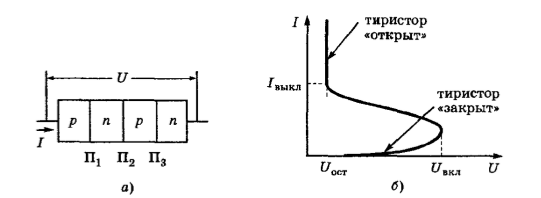
\includegraphics[scale=0.7]{Tir_and_VAH.png}}
		\caption{}	
	\end{figure}
\end{center}

Тиристор можно представить двухтранзисторной моделью:
\begin{center}
	\begin{figure}[h!]
		\center{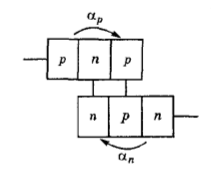
\includegraphics[scale=0.7]{Tir2T.png}}
		\caption{}	
	\end{figure}
\end{center}


Обозначим коэффициент усиления p-n-p транзистора $\alpha_p$, а n-p-n транзистора $\alpha_n$. Ток центрального перехода тиристора П$_2$ складывается из токов коллекторов p-n-p и n-p-n. Если ток во внешней цепи равен I, то до центрального перехода дойдёт ток $\alpha_pI + \alpha_nI$. По условию непрерывности тока, суммарный ток через центральный переход должен быть равен $I$. Если сумма коэффициентов < 1, то через переход П$_2$ должен протекать дополнительный ток, совпадающий по направлению с током во внешней цепи и равный $(1-\alpha_p - \alpha_n)I$. Такое протекание тока соответствует обратному смещению перехода П$_2$ и закрытому состоянию тиристора. Если сумма коэффициентов >1, то через переход должен протекать ток, но уже противоположный по направлению току внешней цепи. Это соответствует открытому состоянию тиристора. При этом на тиристоре падает напряжение, примерно равное падению на обычном p-n переходе. Именуется остаточным напряжением
$U_{ost} \approx 0.7-1.0$В. Известно, что коэффициенты усиления биполярных транзисторов увеличиваются при увеличении тока эмиттера. поэтому при возрастании тока во внешней цепи тиристора сумма коэффициентов увеличивается от значения <1 до значения >1. При этом напряжение на тиристоре сначала возрастает, потом уменьшается. 

Ток выключения $I_{off}$ соответствует условию $\alpha_pI + \alpha_nI = 1$.

Если в область базы n-p-n транзистора втекает внешний управляющий ток, то условие равенства суммы коэффициентов передачи единице выполняется при меньших токах во внешней цепи => меньше напряжение включения. Это называется уже кремниевым управляемым вентилем. Вольтамперные характеристики:

\begin{center}
	\begin{figure}[h!]
		\center{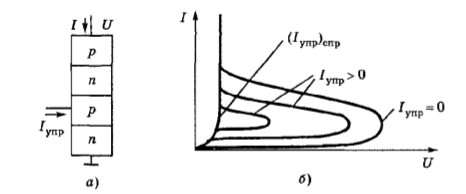
\includegraphics[scale=0.7]{tirI.png}}
		\caption{}	
	\end{figure}
\end{center}

Работа тиристора:
\begin{center}
	\begin{figure}[h!]
		\center{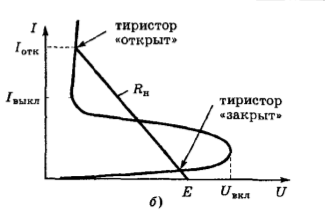
\includegraphics[scale=0.7]{tirworking.png}}
		\caption{}	
	\end{figure}
\end{center}

Рассмотрим включение тиристора в цепь с источником напряжения и нагрузкой R. Предположим, что линия нагрузки пересекает ВАХ тиристора в трёх точках. В закрытом состоянии на тиристоре падает напряжение питания E, так как ток через него очень мал. Переход из закрытого в открытое состояние может произойти вследствие подачи управляющего импульса. Тогда тиристор откроется и останется в состоянии "открыто".

Так как переходы П$_1$ и П$_3$ смещены в прямом направлении, из них в области баз инжектируются носители заряда: дырки из области $p_1$ и элекроны из области $n_2$. Эти носители аряда, диффундируя в областях баз, приближаются к коллекторному переходу и его полем перебрасываются через p-n переход. Дырки, инжектированные из $p_1$ и электроны из $n_2$ движутся через П2 в противоположных направлениях, создавая общий ток I.

При малых значениях внешнего напряжения всё оно практически падает на переходе П2. Поэтому к переходам П1 и П3, имеющим малое сопротивление, приложена маленькая разность потенциалов и диффузия невелика. В этом случае ток через переход равен приблизительно $I_{k0}$. 

Таким образом, свойствами тиристора являются:
\begin{itemize}
\item падение напряжения около 1 В в открытом состоянии. При этом ток может достигать кА.
\item скачкообразный переход по ВАХ
\item $t_{on} << t_{off}$ Обусловлено тем, что заряды, накопившиеся в коллекторе, убираются за счёт рекомбинации в простых тиристорах. Если КУВ => ток управляющий может еще помогать с этой задачей.(источник не указан)
\item имеет участок с отрицательным дифференциальным сопротивлением.

\end{itemize}

Тиристор позволяет использовать часть подаваемой мощности. Тиристорный ключ может проводить в 1 направлении, а в закрытом состоянии способен выдерживать большое прямое и обратное напряжение. 
\begin{center}
	\begin{figure}[h!]
		\center{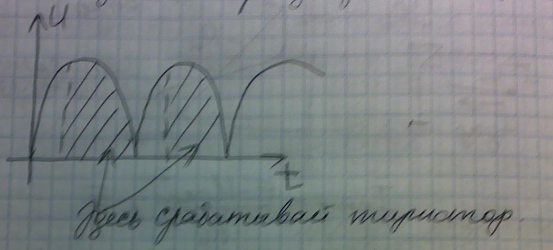
\includegraphics[scale=0.7]{TirLamp}}
		\caption{}	
	\end{figure}
\end{center}

Здесь видно, что тиристор срабатывает на определенном значении входного напряжения. Но выключается не сразу, требуется время $t_{off}$, чтобы он избавился от накопившегося заряда. Поэтому не сразу он переходит в закрытый режим.
